% Bo Ning's simulation-blueprint report style.
\documentclass[lang=en,11pt,a4paper,bibend=bibtex]{elegantpaper}
\usepackage{xeCJK}
\setCJKmainfont{FandolSong-Regular.otf}
\setCJKsansfont{FandolSong-Regular.otf}
\setCJKmonofont{FandolSong-Regular.otf}
\usepackage{tikz,pgfplots,tabularx,titlesec,fancyhdr}
\usetikzlibrary{arrows.meta,positioning,calc}
\pgfplotsset{compat=1.18}
\geometry{left=23mm,right=23mm,top=21mm,bottom=22mm,headheight=15pt,headsep=7mm}
\linespread{1.10}
\setlength{\parindent}{0pt}
\setlength{\parskip}{5pt}
\setlength{\emergencystretch}{2em}
\definecolor{accent}{HTML}{234D64}
\definecolor{muted}{HTML}{59646C}
\definecolor{light}{HTML}{F0F4F6}
\hypersetup{colorlinks=true,linkcolor=accent,urlcolor=accent}
\titleformat{\section}{\Large\sffamily\bfseries\color{accent}}{\thesection}{0.6em}{}
\titleformat{\subsection}{\normalsize\sffamily\bfseries}{\thesubsection}{0.6em}{}
\titlespacing*{\section}{0pt}{9pt}{8pt}
\titlespacing*{\subsection}{0pt}{8pt}{3pt}
\pagestyle{fancy}
\fancyhf{}
\fancyhead[L]{\small\sffamily\color{muted}EXPERIMENT 2\enspace /\enspace ROBOMASTER EP}
\fancyhead[R]{\small\sffamily\color{muted}\studentname}
\fancyfoot[L]{\small\sffamily\color{muted}\studentid\quad\textbullet\quad Individual laboratory report}
\fancyfoot[R]{\small\sffamily\thepage}
\renewcommand{\headrulewidth}{0.3pt}
\renewcommand{\footrulewidth}{0pt}
\captionsetup{font=small,labelfont=bf,labelsep=period,skip=5pt,hypcap=false}
\renewcommand{\arraystretch}{1.18}
\newcolumntype{Y}{>{\raggedright\arraybackslash}X}
\newcommand{\code}[1]{{\small\nolinkurl{#1}}}
\newcommand{\source}[1]{{\small\color{muted}Source: #1}\par}
\newcommand{\reportnote}[1]{\par\smallskip\noindent\colorbox{light}{\parbox{\dimexpr\linewidth-2\fboxsep}{\small #1}}\par\smallskip}
\newcommand{\reporttitle}[1]{\vspace*{2mm}{\small\sffamily\bfseries\color{accent}FIXED-POINT PICK-AND-PLACE}\par\vspace{2mm}{\LARGE\sffamily\bfseries #1\par}\vspace{3mm}{\large\studentname\enspace\studentcn}\par{\small Student ID: \studentid\quad |\quad Individual report}\par\vspace{3mm}\hrule\vspace{3mm}}
\tikzset{box/.style={draw=accent,fill=light,rounded corners=2pt,align=center,font=\small,minimum height=9mm},arr/.style={-{Latex[length=2mm]},thick,draw=accent}}
\newcommand{\teamtable}{%
\par\smallskip
\begingroup\small\renewcommand{\arraystretch}{1.08}
\begin{tabularx}{\linewidth}{@{}>{\raggedright\arraybackslash}p{25mm}>{\raggedright\arraybackslash}p{21mm}Y@{}}\toprule
Member & Work area & Main responsibility \\\midrule
Ning Bo & Simulation & Set up the environment and scene; load models and launch the simulation.\\
Huang Junbiao & Simulation & Work on the motion program and debug grasping, transfer and repeated cycles.\\
Qi Yongyue & Simulation results & Organize logs, analyse results and prepare report material.\\
Bao Lintai & Hardware & SDK communication, task sequence, chassis turn/return and exception handling; joint trials.\\
Xue Yutong & Hardware & Pick/release waypoints, approach/lift heights, gripper adjustment and retention checks; joint trials.\\\bottomrule
\end{tabularx}\par\endgroup}
\newcommand{\commonrequirements}{%
\section{Experiment requirements and individual scope}
The experiment develops a fixed-point grasping task without visual localization: home, approach A, descend, grip, lift, transfer to B, release and return. The course requires a complete simulation launch, state publication, saved trajectories/results/errors, joint and reachability checks, and at least four successful transfers in five consecutive trials. Hardware verification additionally requires supervised low-speed operation, safe failure handling and individual safety-operation checks [1].

Because of equipment availability, our group used the DJI RoboMaster EP arm and gripper instead of the specified mechArm 270. The simulation uses ROS 2 Humble, Gazebo Fortress and custom kinematics/control on a Jetson Linux system. The physical implementation uses the RoboMaster Python SDK. This is a platform adaptation, not an unchanged ROS 2 hardware backend.
}
\newcommand{\commonlimits}{%
\reportnote{Scope of evidence. Simulation repeats A$\rightarrow$B and verifies home after every cycle; the object is reset only between cycles. Hardware alternates A/B, pauses for human grasp confirmation and returns home after all five cycles. Shared ROS 2 interfaces, parameter-only hardware switching and each member's safety check are not demonstrated by the supplied records.}}
\newcommand{\mainresults}{%
\begin{center}\small
\begin{tabular}{@{}crrrcc@{}}\toprule
Cycle & Error (mm) & Heading ($^\circ$) & Time (s) & Placed & Home \\\midrule
1 & 2.274 & 0.445 & 67.01 & Yes & Yes\\
2 & 5.604 & 0.329 & 59.72 & Yes & Yes\\
3 & 4.192 & 0.404 & 60.92 & Yes & Yes\\
4 & 4.577 & 0.459 & 61.09 & Yes & Yes\\
5 & 5.144 & 0.405 & 61.29 & Yes & Yes\\\bottomrule
\end{tabular}
\end{center}
\source{Recorded simulation run \code{20260913_153855_682865/results.json}; error is horizontal distance from configured B, heading is absolute home-heading error.}}
\newcommand{\hardwareresult}{%
\subsection{Physical validation: team-observed outcome}
The team confirmed that all five hardware transfers succeeded with no observed abnormalities. Cycles 1, 3 and 5 moved A$\rightarrow$B; cycles 2 and 4 moved B$\rightarrow$A. Each lift was followed by a fresh human \code{y} confirmation before rotation; final heading restoration and homing followed cycle 5. This is an observed 5/5 result, not an instrumented precision or timing measurement. No real-hardware position-error, duration or force data are available, and five successes do not establish long-run reliability.}
\newcommand{\githubsection}{%
\clearpage
\section{Shared GitHub repository and commit evidence}
The complete group archive is stored in the
\href{https://github.com/ccx8kg5qpd-debug/robomaster-ep-fixed-point-grasping}
{shared public GitHub repository}. The repository address is
\nolinkurl{github.com/ccx8kg5qpd-debug/robomaster-ep-fixed-point-grasping}.
It contains the simulation and hardware programs, model resources, saved results,
the complete simulation recording and all five individual report sources.

\begin{center}
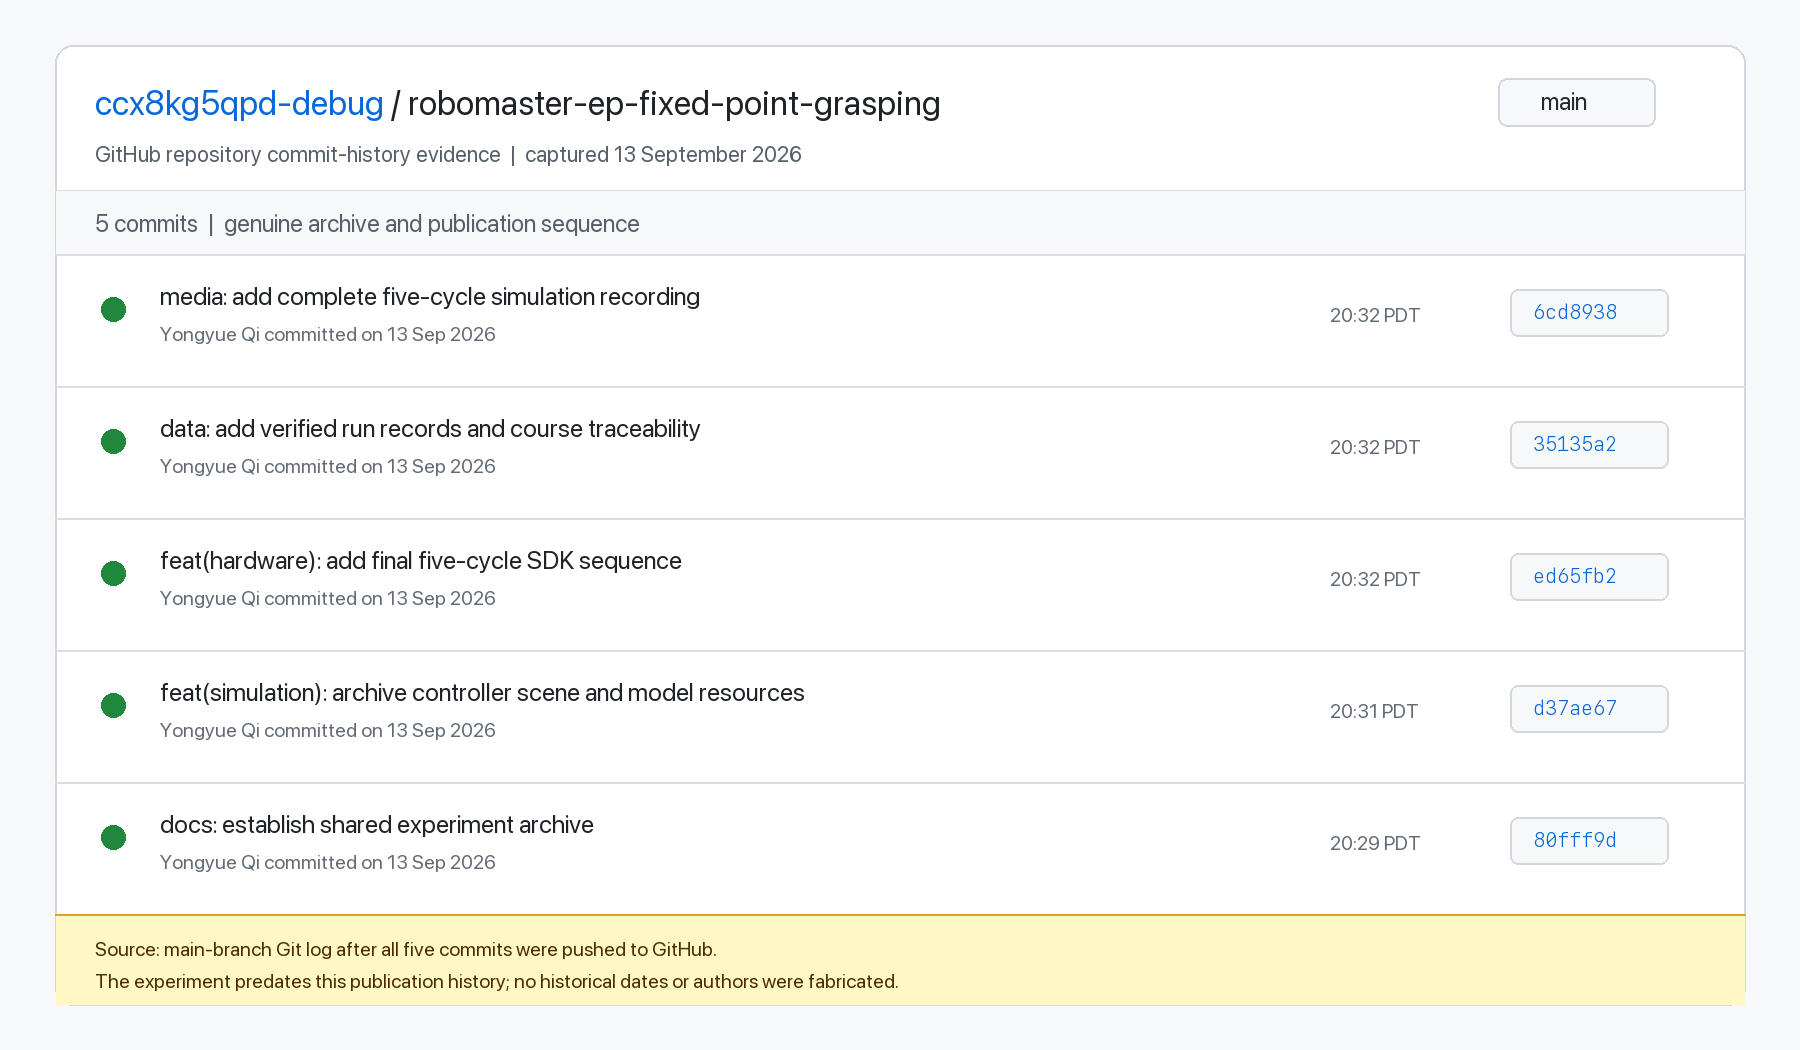
\includegraphics[width=\linewidth]{assets/commit_history_snapshot.png}
\captionof{figure}{Commit-history evidence captured after the first five project
materials commits had been pushed to the shared GitHub repository.}
\end{center}

\reportnote{Traceability note. The experiment was completed before the GitHub
repository was assembled. These genuine commits document the later review,
organization and publication sequence; they are not presented as a fabricated
contemporaneous development history. The screenshot records the five commits
visible at capture time, before this revised report was added.}
}
\newcommand{\referencesblock}{%
\section*{Sources and traceability}
{\footnotesize
[1] Course handout, \emph{Fixed-Point Robotic-Arm Grasping: Simulation Development and Hardware Validation}, S16--S20 / E5; individual-report assignment requirements.\par
[2] Shared team repository, \href{https://github.com/ccx8kg5qpd-debug/robomaster-ep-fixed-point-grasping}{robomaster-ep-fixed-point-grasping}, assembled 13 September 2026: simulation source/configuration, \code{real_v2_five_cycles_manual.py}, saved logs and reports. Primary numerical record: \code{20260913_153855_682865}.\par
[3] Team conversation fact-check materials, 13 September 2026, for development history; subsequent team confirmation for the completed five-cycle hardware run. Historical failures are not counted as final-run failures.\par
[4] Community model resources: \href{https://github.com/jeguzzi/robomaster_ros}{jeguzzi/robomaster\_ros}, archived commit \code{c05a39d7f0fa}. Report layout uses \href{https://ctan.org/pkg/elegantpaper}{ElegantPaper}, distributed under LPPL 1.3c.
}}

\definecolor{accent}{HTML}{005A73}
\definecolor{muted}{HTML}{506771}
\definecolor{light}{HTML}{E9F7FA}
\definecolor{gridblue}{HTML}{9DD9E5}
\geometry{left=20mm,right=24mm,top=23mm,bottom=20mm,headheight=16pt,headsep=6mm}
\hypersetup{linkcolor=accent,urlcolor=accent}
\titleformat{\section}{\Large\sffamily\bfseries\color{accent}}{\thesection}{0.7em}{}[\color{gridblue}\titlerule]
\titleformat{\subsection}{\normalsize\sffamily\bfseries\color{accent}}{\thesubsection}{0.55em}{}
\fancyhead[L]{\small\sffamily\bfseries\color{accent}SIMULATION BLUEPRINT 02}
\fancyhead[R]{\small\sffamily\color{muted}\studentname\ /\ \studentid}
\fancyfoot[L]{\scriptsize\sffamily\color{muted}Scene, model resources and launch integration}
\fancyfoot[R]{\small\sffamily\bfseries\color{accent}\thepage}
\renewcommand{\headrulewidth}{1pt}
\renewcommand{\reportnote}[1]{\par\smallskip\noindent\fcolorbox{gridblue}{light}{\parbox{\dimexpr\linewidth-2\fboxsep-2\fboxrule}{\small\textbf{Blueprint note.} #1}}\par\smallskip}
\renewcommand{\reporttitle}[1]{\vspace*{1mm}\noindent\colorbox{accent}{\parbox{\dimexpr\linewidth-2\fboxsep}{\color{white}\sffamily\small\bfseries SIMULATION / ENVIRONMENT / SCENE}}\par\vspace{5mm}{\fontsize{23}{27}\selectfont\sffamily\bfseries\color{accent}#1\par}\vspace{3mm}{\large\sffamily\studentname\enspace\studentcn\par}{\small Student ID \studentid\quad|\quad Individual design: simulation blueprint}\par\vspace{4mm}{\color{gridblue}\rule{\linewidth}{2pt}}}

\newcommand{\studentname}{Ning Bo}
\newcommand{\studentcn}{宁博}
\newcommand{\studentid}{24020036049}
\begin{document}
\reporttitle{Simulation Setup\\and Scene Construction}
\commonrequirements
\subsection{My responsibility and team interfaces}
My main responsibility is preparing the simulation environment and scene: loading the RoboMaster model, arranging the table and cube, checking resource paths and starting the simulation. I coordinate with Huang Junbiao on model or scene problems that affect his motion-program debugging, and provide the final scene/configuration material to Qi Yongyue for result analysis. Bao Lintai and Xue Yutong handle the physical experiment. This report focuses on getting a usable simulated setup ready for repeated grasping.
\teamtable
\commonlimits
\clearpage
\section{Scene geometry and physical assumptions}
\subsection{A common support plane}
The world file places the robot and object on a shared table. Its box geometry is $1.6\times1.2\times0.05$ m, with centre height 0.035 m, giving a top surface at $z=0.060$ m. The object is a 0.025 m cube, so its resting centre should be $0.060+0.0125=0.0725$ m. It is spawned at 0.0735 m, 1 mm above that equilibrium height, and settles under the physics engine.
\begin{center}
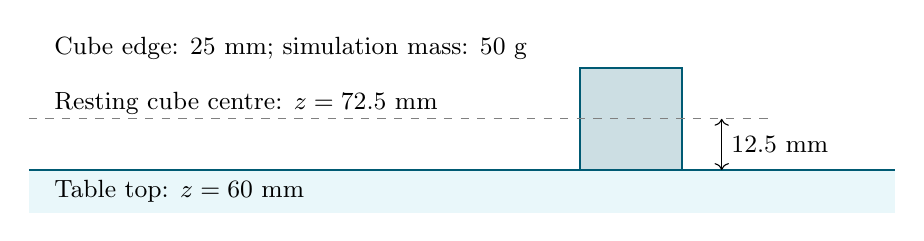
\begin{tikzpicture}[x=1cm,y=1cm]
\fill[light] (0,0) rectangle (11,.55);
\draw[accent,thick] (0,.55)--(11,.55);
\draw[fill=accent!20,draw=accent,thick] (7,.55) rectangle (8.3,1.85);
\draw[dashed,gray] (0,1.2)--(9.4,1.2);
\draw[<->] (8.8,.55)--node[right,font=\small]{12.5 mm} (8.8,1.2);
\node[anchor=west,font=\small] at (.2,.28){Table top: $z=60$ mm};
\node[anchor=west,font=\small] at (.2,1.4){Resting cube centre: $z=72.5$ mm};
\node[anchor=west,font=\small] at (.2,2.1){Cube edge: 25 mm; simulation mass: 50 g};
\end{tikzpicture}
\captionof{figure}{Height consistency in the world frame; schematic, not to scale.}
\end{center}
The fixed object-centre targets are $A=(0.278,-0.001,0.0725)$ m and $B=(0.237,0.1453,0.0725)$ m. The A/B markers are visual references, not collision platforms. Therefore, their appearance must not be interpreted as two elevated support pads. Contact with the actual table is checked when accepting a placement.
\subsection{Mass and inertia}
The simulation assigns mass $m=0.05$ kg to the cube. For a uniform cube of edge $a=0.025$ m, the principal moments are
\begin{equation}
I_{xx}=I_{yy}=I_{zz}=\frac{ma^2}{6}=5.2083\times10^{-6}\ \mathrm{kg\,m^2}.
\end{equation}
This is a model parameter, not a measured mass of the real object. The handout limits the real target to 100 g, but no measured physical mass is supplied. I would not claim that the 50 g simulation setting proves compliance of an unweighed real target.
\subsection{Frames matter as much as dimensions}
The kinematic model incorporates a 0.060 m base-height offset. Its home/hover/grasp tip coordinates are consequently not raw clearances above the tabletop. Mixing these coordinates with world object-centre coordinates, or with SDK millimetres, would create a systematic height error even if every numerical value were copied correctly.
\clearpage
\section{Model resources and integration}
\subsection{Visual meshes, collision meshes and link frames}
The robot model uses the community \code{robomaster_description} resources bundled with the project [4]. Visual geometry determines appearance; collision geometry determines physical interaction. The controller also relies on the model's link/joint transforms to locate the fingertips. These three uses of the model must agree on frame origins and scale.

The supplied kinematics explicitly identifies the forward end of gripper link 4 as the grasping region; link 7 is a rear linkage rather than a fingertip. This distinction explains why choosing a link by its number or visual prominence is unsafe. An apparently reasonable end-effector reference can still be located at the wrong part of the mechanism.
\begin{center}
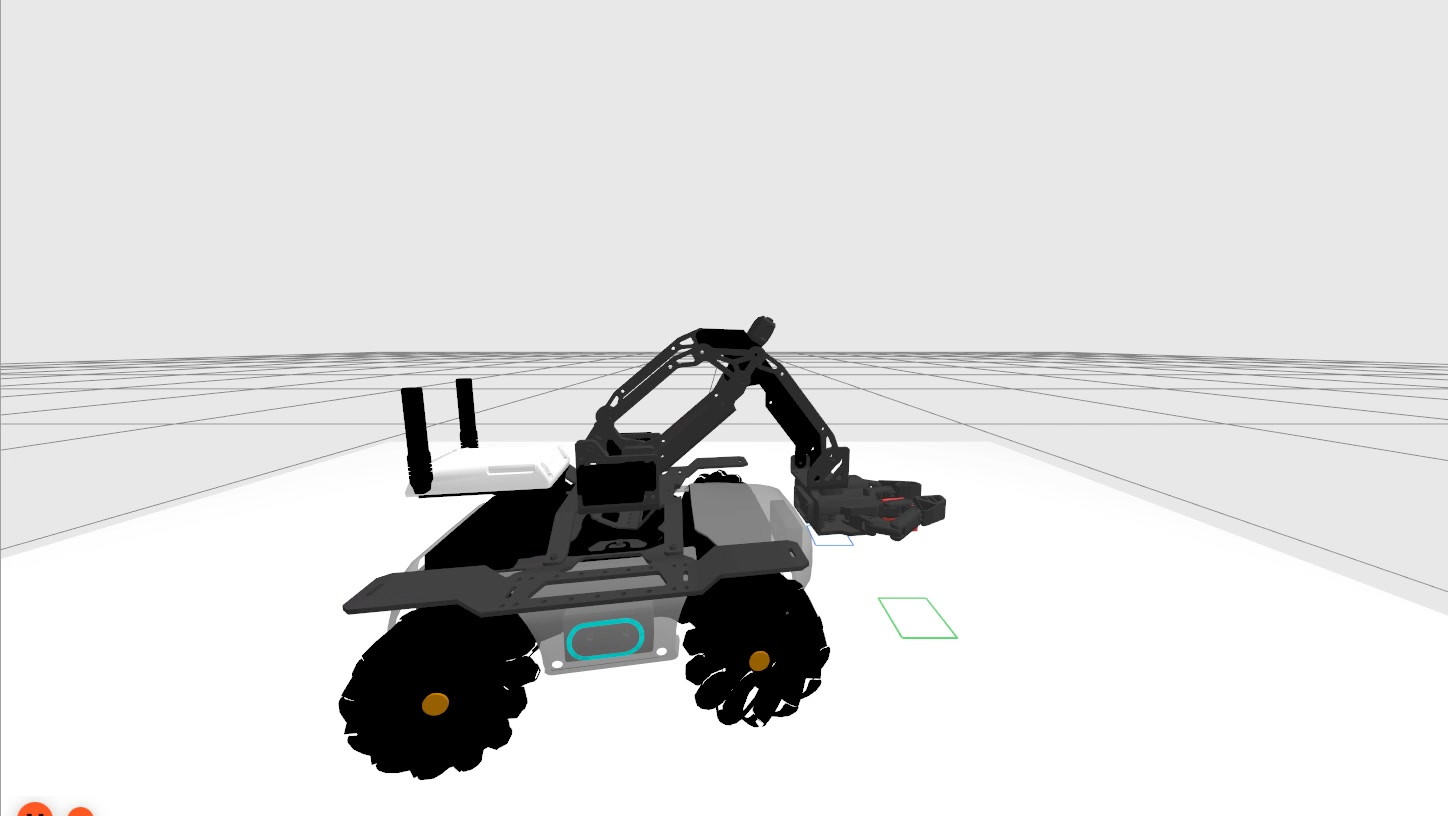
\includegraphics[width=.87\linewidth,trim=0 20 0 230,clip]{assets/lift.jpg}
\captionof{figure}{Scene frame from the team's simulation recording at 34 s. The image documents model context, not real-hardware accuracy.}
\end{center}
\subsection{Making the archived model portable}
Earlier development notes describe missing mesh resources and fragmented model appearance. The final archive includes the complete dependency directory and \code{prepare_paths.py}, which creates a runtime copy with resource paths adjusted to the bundled model. This is more reproducible than assuming another computer has the author's original absolute Linux paths.
\begin{center}\small
\begin{tabularx}{\linewidth}{@{}p{42mm}Y@{}}\toprule
Component & Function and dependency\\\midrule
\code{ep_feedback.world.sdf} & Table, target cube, markers and world systems.\\
\code{ep_feedback.sdf} & Robot links/joints, collisions and control plugins.\\
\code{robomaster_description} & Mesh resources required by the archived model.\\
\code{ep_kinematics.py} & Frame reconstruction and fingertip-centre calculation.\\
\code{ep_transfer.launch.py} & Starts simulator, bridge, spawn and task nodes.\\\bottomrule
\end{tabularx}
\end{center}
\subsection{Starting the complete simulation}
The startup wrapper sources ROS 2 Humble and the workspace environment. One launch file starts Gazebo, the bridge and refill node, schedules robot creation after 5 s and starts the task controller after 8 s. When preparing a run, the important checks are that the robot and cube have loaded and that joint/pose feedback is available. The fixed startup delays are not themselves proof of readiness; slow model loading can still prevent a task from starting.
\clearpage
\section{Physical validity and observed results}
\subsection{Contact grasping versus scene manipulation}
The final transfer controller uses gripper/object contact rather than continuously attaching or teleporting the cube along a scripted trajectory. Its bilateral-contact test identifies fresh collisions from both gripper sides. The cube must subsequently rise above the configured height condition before transfer continues.

There is nevertheless a legitimate object-position reset in the system: the separate refill node moves the cube back to A after home verification, between cycles 1--4. It is enabled only in \code{REFILL_WAIT}. This operation represents experiment replenishment, not the physical grasping mechanism. Keeping that distinction explicit avoids claiming that every object movement in the world is unmodified physics.
\mainresults
The recorded run completed five placements and five returns home. The maximum horizontal placement error was 5.604 mm; the configured acceptance limit is 23 mm, together with an 8 mm height window and table contact. The settled centre heights near 72.5 mm are consistent with the table-plus-half-cube calculation, providing a useful cross-check of the scene geometry.

These results support a functioning contact-based demonstration under the selected model and parameters. They do not establish mesh-level collision accuracy, realistic friction over all surfaces, or agreement with measured hardware dynamics. A successful placement is a system-level outcome, not an independent validation of every model parameter.
\hardwareresult
\clearpage
\section{Problems, solutions and individual reflection}
\subsection{A complete-looking model can still be wrong}
Missing mesh paths explain invisible parts, while incorrect frame or inertia references can produce a model that renders but behaves incorrectly. The archived solution is a complete resource set and explicit frame reconstruction. My preferred diagnostic order is to check resource resolution, dimensions, frame relationships and physical contact separately. Changing controller gains before checking those foundations risks compensating for a geometry error.
The development notes also record pasted shell formatting and Python-environment problems. Keeping commands in plain scripts, sourcing the intended ROS environment and using the system interpreter helps separate an environment failure from a motion-program failure. This is the handoff point between my setup work and Huang Junbiao's program debugging.
\subsection{Placement regions must match reachable geometry}
Development notes identify unsuitable early placement locations, including a destination conflicting with the vehicle region. The final A/B arrangement uses chassis turning to bring the gripper toward B. A marker's presence is not enough: the reachable fingertip set, chassis footprint and descent corridor must all be compatible. A top-view geometric check should precede a full pick-and-place trial.
\subsection{Clearance checking has a limited scope}
The retrospective materials describe a nine-point geometric audit from $(x,z)=(0.235,0.220)$ m to $(0.270,0.160)$ m at closure 0.6, with no reported intersections at those samples. This is useful local evidence. However, the actual controller interpolates joint angles, so a straight Cartesian sample set is not necessarily the executed path. It also does not examine every link configuration during closing, turning or lowering.

My proposed improvement is to evaluate the actual interpolated joint sequence against the collision model, then repeat with small target and object-size perturbations. Those checks should be reported as additional tests when performed, not retroactively asserted as completed. This would connect static scene validation to the moving mechanism more directly.
\subsection{Main lesson}
Scene building is an engineering task, not just visualization. Consistent support height, fingertip reference, mass/inertia and resource packaging make the downstream controller interpretable. The final five-cycle results are encouraging, but real-world transfer requires measured object properties and hardware calibration. For this report, I keep the 50 g mass, numerical contact behavior and millimetre errors explicitly within the simulation evidence.
\githubsection
\referencesblock
\end{document}
